\documentclass[a4paper,11pt]{jsbook}

\newcommand{\V}[1]{\boldsymbol{#1}}
\def\thline{\noalign{\hrule height 1pt}}
\def\tvline{\vrule width 1pt}

\usepackage{here} %図の場所の指定で[H](ここに貼る)を指定するためのパッケージ
\usepackage{makeidx}
\usepackage{amsmath}
\usepackage{amssymb}
\usepackage[dvipdfmx]{graphicx} %dvipdfmxはjpgやpngの張り込みのために使用


\makeindex

\pagenumbering{roman}

\begin{document}
% 表紙
\title{2019年度 卒業論文\\
\vspace{\baselineskip}
単眼カメラSLAMを完遂する環境要件\\
Environmental requirements to complete\\
 monocular camera SLAM }
\author{千葉工業大学 先進工学部 未来ロボティクス学科\\
学籍番号 16C1096\\
鳴海 和真}




\date{2020年2月7日}

\maketitle

%%% 但し書き等 %%%
\clearpage

\chapter*{謝辞}\addcontentsline{toc}{chapter}{謝辞}

 本研究を進めるにあたり、ご指導を頂いた卒業論文指導教員の上田隆一准教授に感謝いたします。


\tableofcontents

%\cleardoublepage

%%% 本文 %%%
% 章のページの先頭は左側(奇数ページ)に来る

\cleardoublepage
\pagenumbering{arabic}

\chapter{序論}

\section{背景}

Simultaneous Localization and Mapping(以下, SLAM)は、自己位置推定と環境地図の生成を同時に行う技術である。SLAMは、工場で稼働する無人運搬車や自動車の自動運転、ロボット掃除機といった自律行動をするロボットに活用されている\cite{Kondo2019}。中でも、カメラ映像からSLAMを行うものをVisual SLAMという。単眼カメラSLAMはVisual SLAMを単眼カメラのみで行う。単眼カメラSLAMはVisual SLAMの中で最も安価かつ小型で消費電力を抑えられることが長所である\cite{Artal2017}。
\section{問題}

単眼カメラSLAMには、空間把握をカメラ画像に依存するために、エッジや模様のない環境に対して特徴点検出ができなくなるという問題が存在する。このような場合にはSLAMが中断される。この問題の解決策として、IMUやRGB-Dといったセンサを併用することによる方法が一般的である。しかし、この方法ではセンサの高価格化、大型化および消費電力の増加によって前述した単眼カメラSLAMの長所を活かすことができない。

\section{目的}

単眼カメラSLAMを中断されることなく完遂することのできる環境要件を調査することを目的とする。ここでの環境要件とは単眼カメラSLAMが中断されないために最低限必要とされる特徴とする。本目的の達成によってロボットに用いられるセンサのコスト低下、軽量化されることによりSLAM導入のハードルを低下させることができると言える。

\section{本論文の構成}

本論文では、2章で提案手法を述べ、3章で実験の方法と結果を示し、4章で結論を述べる。

% dvipdfmxとhereのテスト
%\begin{figure}[H]
%	\begin{center}
%		\includegraphics[width=1.0\linewidth]{../zero.png}
%		\caption{}
%		\label{fig:}
%	\end{center}
%\end{figure}
%

%\include{purpose}
\chapter{提案手法}\label{chap:method}

\section{問題設定}

今回は、倉庫等特定の環境で稼働するロボットを想定する。予め単眼カメラSLAMを行うロボットの補助のために環境改善が可能であることとする。ここで、環境への影響を最小限に抑えて単眼カメラSLAMが中断する環境を改善する条件を実験により調査する。

\section{解決方法}

単眼カメラSLAMによる特徴点検出ができない環境にマーカを設置することで問題を解決する。このとき、環境への影響が最小限になるようなマーカの範囲を求める。

\chapter{実験}\label{chap:test}

\section{使用機器}

単眼カメラセンサとしてWebカメラLogicool C270を使用する。カメラキャリブレーションを行い歪みを補正する。
SLAMは、カメラSLAMライブラリのORB-SLAM2\cite{Artal32017}を使用。


\section{実験条件}

実験環境として、図\ref{fig:picture01}を用意する。壁面まで距離1[m]、高さ1[m]地点にカメラを設置する。一面には単色無地のカーテンをかける。なぜカーテンを用いるかという特徴点検出の難しい環境の再現に適しているからである。ORB-SLAM2はFASTキーポイント検出\cite{Hujiyosi2011}によりエッジから特徴点検出をする\cite{Artal22017}。この特徴点を追跡(トラッキング)することでカメラの位置姿勢を推定し、三次元空間における座標計算から環境地図生成をする。このため、エッジの立たない物体であるカーテンから特徴点検出をすることはできずORB-SLAM2が中断される。もう一面には棚を配置する。この棚はエッジが十分に検出可能で、ORB-SLAM2によるトラッキングの開始をスムーズにさせる役割を果たす。

\begin{figure}[h]
        \begin{center}
        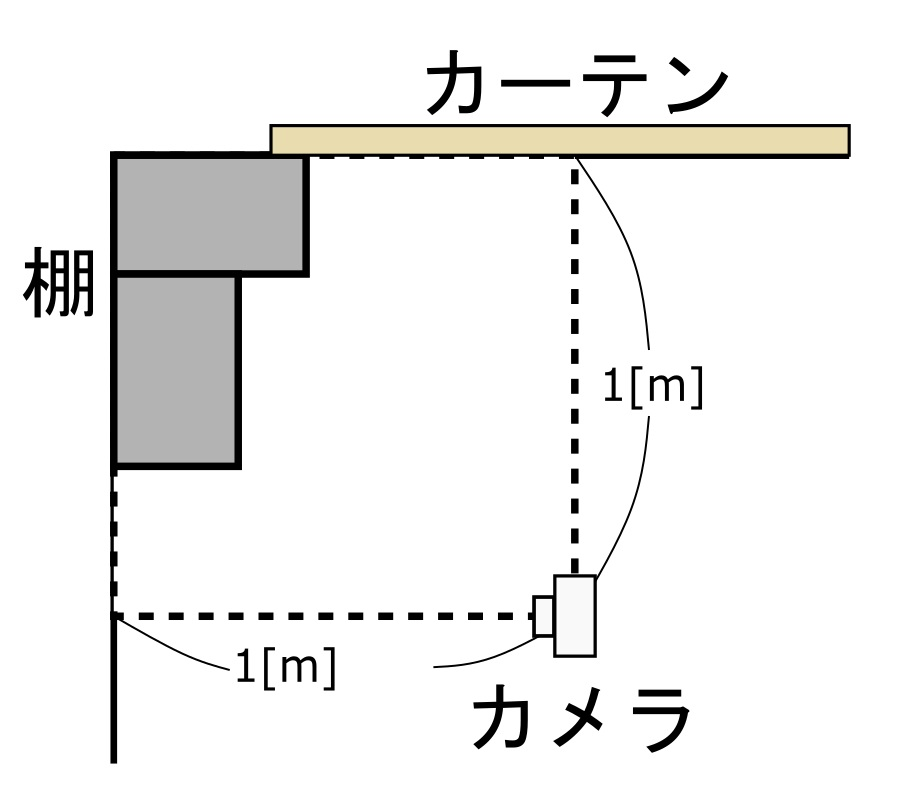
\includegraphics[width=0.35\linewidth]{figs/picture01.jpg}
        \caption{実験環境概略図}
        \label{fig:picture01}
        \end{center}
\end{figure}

\newpage

\section{実験方法}

ORB-SLAM2を起動し、カメラを棚に向けてトラッキングを開始する。カメラをカーテンへ向けていくとやがて特徴点検出ができなくなり、カメラの画角が図\ref{fig:picture02}赤線部となる位置でトラッキングが停止する。カメラ画像が図\ref{fig:Tracking02}となるこの位置よりカーテン方向へカメラを向けるとトラッキングが停止し、SLAMが中断される。

\begin{figure}[h]
 \begin{tabular}{cc}
      \begin{minipage}[t]{0.45\hsize}
        \centering
        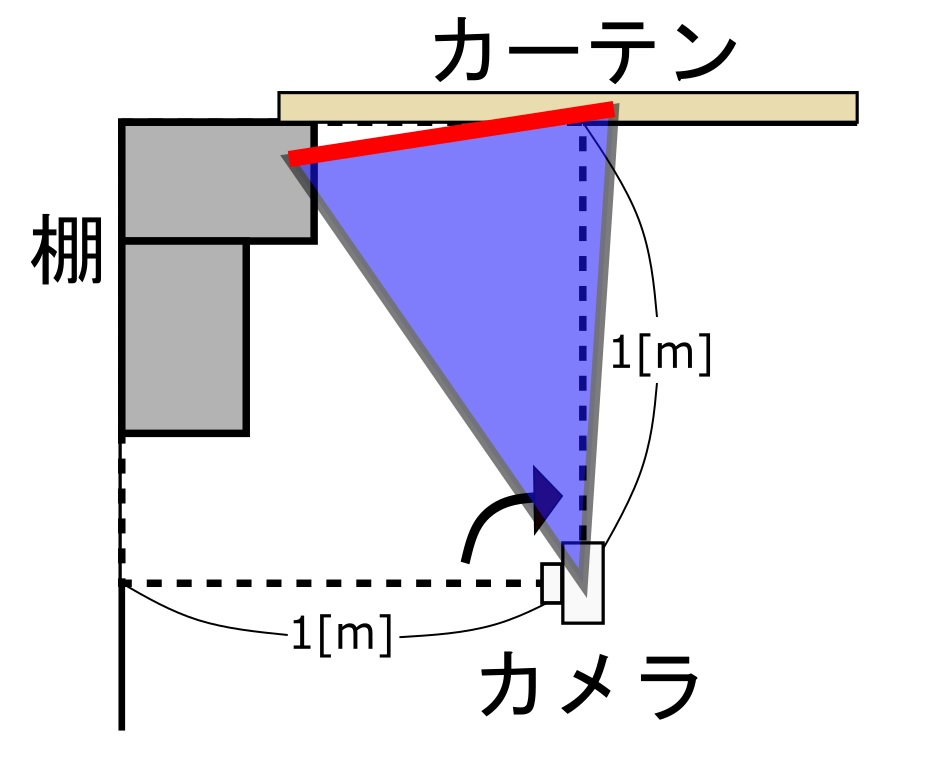
\includegraphics[width=1.0\linewidth]{figs/picture02.jpg}
        \caption{実験概略図}
        \label{fig:picture02}
        \end{minipage} &

      \begin{minipage}[t]{0.45\hsize}
        \centering
        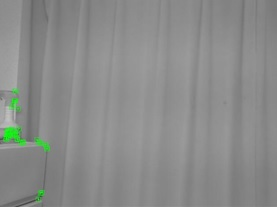
\includegraphics[width=1.0\linewidth]{figs/Tracking02.jpg}
        \caption{図\ref{fig:picture02}赤線部のカメラ画像}
        \label{fig:Tracking02}
  \end{minipage}

 \end{tabular}
\end{figure}

ここでトラッキングを継続させるためにマーカを使用する。本実験では直径19.5[mm]のシールをマーカとして使用する。

\begin{figure}[h]
        \begin{center}
        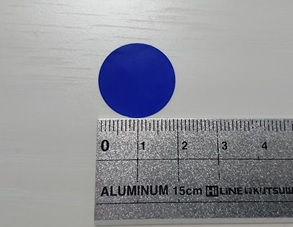
\includegraphics[width=0.6\linewidth]{figs/marker01.jpg}
        \caption{マーカとして使用するシール}
        \label{fig:marker01}
        \end{center}
\end{figure}

\newpage

トラッキング継続に必要なマーカを絞り込むための手順を以下に示す。


\begin{enumerate}
   \item カメラからの距離1[m],高さ1[m]地点のカーテン表面を中心にマーカを貼り付ける。
   \item マーカのみをトラッキングするようにカメラをカーテン方向へ回転する。
   \item マーカを100[mm]間隔で縦方向に増やす。SLAMを再起動し再び手順2を行う。これをトラッキング可能になるまで繰り返す。
  \item マーカの間隔を10[mm]狭める。SLAMを再起動し再び手順2を行う。これをトラッキング不能になるまで繰り返す。
  \item マーカの間隔を1[mm]広げてSLAMを再起動し2を行う。これをトラッキング可能になるまで繰り返す。
   \item マーカの間隔と特徴点マッチング数を記録する。
\end{enumerate}

\begin{figure}[h]
        \begin{center}
        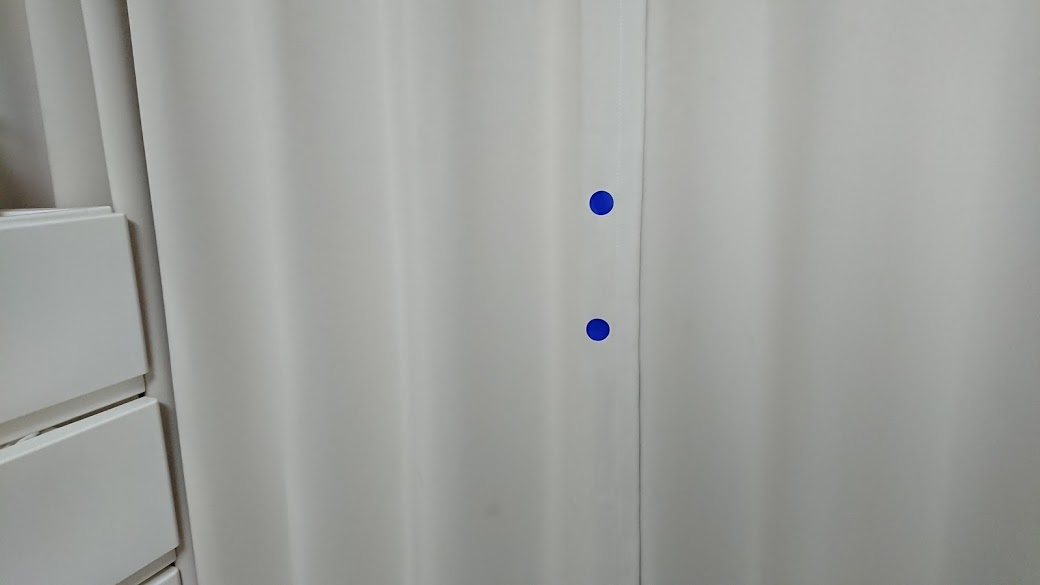
\includegraphics[width=0.7\linewidth]{figs/marker03.jpg}
        \caption{カーテン表面に貼付されたマーカ}
        \label{fig:marker03}
        \end{center}
\end{figure}

\newpage

\section{実験結果}

シール1〜3枚をマーカとしたときはトラッキング不能であった。シール4枚をマーカとした時にマッチング可能となった。さらにマーカの間隔を狭めたときの特徴点マッチング数を表\ref{table:matching value}に示した。マーカ間隔47[mm]までは特徴点マッチング数95〜121を獲得しトラッキングは安定していた。46[mm]になると特徴点の消失と復帰を繰り返す不安定な動作となった。以上より、本実験では47[mm]間隔で配置された4枚のシールが単眼カメラSLAMを完遂できる最小範囲のマーカとなった。

\begin{table}[htb]
\begin{center}
  \caption{記録したマーカ間隔と特徴点マッチング数}
  \label{table:matching value}
  \begin{tabular}{|c||c|} \hline
	マーカ間隔[mm] & 特徴点マッチング数 \\ \hline \hline
	46 & Lost〜78 \\ \hline
	47 & 95〜121 \\ \hline
  \end{tabular}
\end{center}
\end{table}

\begin{figure}[h]
        \begin{center}
        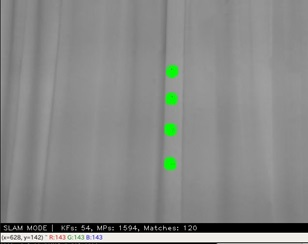
\includegraphics[width=0.7\linewidth]{figs/Tracking03.jpg}
        \caption{マーカのみでトラッキング継続成功}
        \label{fig:Tracking03}
        \end{center}
\end{figure}


\chapter{結論}

単眼カメラSLAMを完遂するために必要な特徴点マッチング数を絞り込む手法を提案した。同様の手順を行うことで単眼カメラSLAMを完遂できない環境を最小限のマーキングによって改善可能である。
課題点として、本研究の実験方法はトラッキングが開始されることを前提にしている点が挙げられる。実験において棚に該当する特徴点検出が容易な物体を隣接していない環境では同じ手法では不十分である。この課題の解決には新たな実験条件を考案する必要がある。




%\appendix


%%%参考文献%%%
% よほどのことが無い限りet al.は使わないことにしましょう
\bibliographystyle{jualpha}
\bibliography{./references}

\newpage
\printindex

\end{document}


